\documentclass[11pt, a4paper]{article}
\usepackage[UKenglish]{babel}
\usepackage[bibstyle=ieee, dashed=false, sorting=nty]{biblatex}
\usepackage[labelfont=bf]{caption}
\usepackage{csquotes}
\usepackage{fancyhdr}
\usepackage{float}
\usepackage{graphicx}
\usepackage[top=25mm, right=20mm, bottom=25mm, left=20mm]{geometry}
\usepackage[hidelinks]{hyperref}
\usepackage{microtype}
\usepackage{parskip}
\usepackage[small,compact]{titlesec}

\titlespacing*{\section}{0pt}{\baselineskip}{0.35\baselineskip}

\pagestyle{fancy}
\fancyhf{}
\fancyhead[L]{COM3504}
\fancyhead[C]{The Intelligent Web: Assignment}
\fancyhead[R]{Team: Gakki}
\fancyfoot[C]{\thepage}

\addbibresource{references.bib}

\begin{document}
\section{Introduction}
Progressive Web App (PWA) allows users to create and comment on both events and user stories.
Social media features such as `like', `follow', `interested', and `going' were integrated. Users are
able to tag an event with their stories, which will then appear in the `Explore' page. Users can
create a story by taking a picture with their front camera through the use of WebRTC or upload a
picture locally. Each user story can receive likes and comments, for which the latter was
implemented using Socket.IO \cite{week6, socketio}. Socket.IO was also used for posting comments in
the `Discussion' of each event. Service worker was implemented to cache requests for offline usage.
MongoDB was used to store and synchronise data between the client and server, while IndexedDB was
used to store data loaded from MongoDB for offline usage. However, data stored in MongoDB can only
be retrieved when user is online. The search function (via location) was implemented with Google
Maps API, allowing autocomplete for the location field and ensuring that a valid location is used.
For security purposes, users can only login with their respective Google Account.

\section{Diagrams}
Appendix \hyperref[figure:site_map]{\textbf{Figure 1}} and Appendix \hyperref[figure:uml]{
\textbf{Figure 2}} are the detailed description of the PWA system structure.
\hyperref[figure:site_map]{\textbf{Figure 1}} describes the interactions between the front-end,
data storage, caching and data retrieval. Functionalities are limited and users are unable to have a
personalised user experience if sign-in through Google Account is not completed. Data is retrieved
from MongoDB and stored in IndexedDb when server connection is available. This enables user to
access preloaded information when they are offline. Caching takes place with the use of service
workers when users are online. \hyperref[figure:uml]{\textbf{Figure 2}} demonstrates the database
model along with the relationship between documents. The types of data collected for each document
and the functions used for data retrieval are also described.

\section{Interface to Insert and Search Data via Forms}
\textbf{Challenges:} Search speed must be efficient and search results must be accurate with respect
to the given query. Users must be able to search for events, stories, and profile of other users.
Basic text search will allow users to input any text query and return the results sorted by
relevance. Users can use partial words to search for an event or profiles of other users.
Advanced search will allow users to search for events based on event name, genres, venue (address)
and date. When creating an event, Place Autocomplete by Google Maps API \cite{google_maps_api} is
used to provide users with valid locations as options. \textbf{Solution:} FlexSearch.js
\cite{flexsearch} was chosen to implement basic text searching task due to its efficient,
lightweight, and flexible properties \cite{flexsearch_benchmarkk}. It allows multi-field search and
accepts multiple data format types as data index. Hence, it is used with both MongoDB and IndexedDB
to provide searching functionality in both online and offline environment respectively. This was
implemented for both searching for events and stories, where user provides relevant input and
are given resulted options sorted by relevance (most relevant on top) in a drop-down menu.
Users are able to search for events via event name, location/address, genre, and date of event.
Users can search for stories via event name, tagged location/address, and date posted. This allows
users to post stories related to an event from another location (not restricted to the event
location) and they are able to post throwbacks (not restricted to date and time of event occurrence).
\textbf{Requirements:} Users should be able to search for events and user profiles while online and
offline. Users should be able to obtain results through querying with partial information. The
results returned are sorted by relevance. \textbf{Limitations:} On every page load, the data has to
be retrieved from IndexedDB to populate the FlexSearch.js's search index. The performance loss might
be negligible when the total data size is small, but it may cause longer loading time when the size
of data exceeds a certain size. Google Maps API request could not be cached as it generates a random
token for every request made, hence Place Autocomplete will not work offline.

\section{Interface to Search Data via Map}
\textbf{Challenges:} The use of map with accurate location where caching is able to take place.
Custom marker is placed on the location of the event. Multiple markers would cause stacking, leading
to confusion and poor user experience. \textbf{Solutions:} Map was implemented with Leaflet Geocoder.
In the implementation of searching for events, markers are placed to display pop-up of image and
link of ongoing and future events upon clicking, while in the implementation of searching for
stories, markers are placed to display pop-up of image, username and caption of stories upon clicking.
Offline searches will display marker on cached location of event. To handle stacking of multiple
markers (multimarker), Leaflet Marker Cluster was used. This would result in number of markers
of each cluster to be displayed. Upon clicking, each marker would be displayed. \textbf{Requirements:}
Allow users to search for events using a map in both online and offline environments. Past events 
should not appear on the map. Future and ongoing events should be displayed as custom markers on the
map. Custom markers should pop-up to display the event information when clicked. \textbf{Limitations:}
The map takes time to load and does not generate immediately. Google Maps API was not chosen to be
implemented in this task as request could not be cached due to the generation of random token for
every request made, making it unavailable when user is offline. Caching the map tiles consumes more
storage than other requests as map tiles are stored as images. If Place Autocomplete by Google Maps
API \cite{google_maps_api} was not implemented, users would be able to insert invalid locations,
causing markers of any previously created events with valid locations to not show up on the map.
Hence, heavily relies on the input to be of valid locations. When there exist multiple markers, E.g.
20 or more, on the exact same location, stacking of markers will occur. Markers are loaded all at
once regardsless of whether or not the marker is within the frame of screen. This could be handled
with the implementation of lazy loading, but is not implemented in the current site due to time
constraint.

\section{PWA – Caching of the App Template Using a Web Worker}
\textbf{Challenges:} Fetching cross-domain response will result in an opaque response, which will
consume huge storage quota compared to normal responses \cite{opaque_workbox}. Sending a fallback
offline page response when user is offline and visit a page that does not exist in the cache.
\textbf{Solutions:} `Cache then network' was used and modified according to The Offline Cookbook
\cite{offline_cookbook}. \textbf{Requirements:} Users should be able to view a basic offline
template with required data when page was not visited in the past and user is offline. Users should
be able to view previously loaded events, stories, and profiles without the ability to make any
changes. \textbf{Limitations:} Non-static files are not cached in the installation stage
of the service worker. Page that has never been visited before will not be cached. This applies to
events or stories which were updated, where instead of the updated information, the cached
information, which might not be up-to-date, will be displayed when user is offline.

\section{PWA: Caching Data Using IndexedDB}
\textbf{Challenges:} Retrieve data from MongoDB and store them in IndexedDB. Display page content
using data loaded from IndexedDB when no internet connection is present. \textbf{Solution:} Retrieve
data from MongoDB using AJAX. Promise is used for both storing and loading of data from IndexedDB.
\textbf{Requirements:} Data on events and user profiles must be stored locally for offline searching.
Users should be able to access data retrieved from IndexedDB when they are offline.
\textbf{Limitations:} A known bug of IndexedDB storage is usage increases with every $put()$
operation \cite{leveldb_593, leveldb_603}.

\section{NodeJS Server Including Non-Blocking Organisation of Multiple Dedicated Servers}
\textbf{Challenges:} Uses asynchronous functions to handle file upload, data retrieval from server,
or other function calls that require time to complete. Errors might occur during the execution
of asynchronous functions. \textbf{Solution:} Uses the Promise and async/await features of
JavaScript to handle both successful and failed function operations. Keep the code nesting shallow
to make code more maintainable and readable. \textbf{Requirements:} Able to use Promise to order the
sequence of asynchronous processes. Able to use callbacks to handle the success and failure of
asynchronous functions. \textbf{Limitations:} Single threaded mechanism, not suitable for
CPU-intensive operations. Relies heavily on callbacks, which might possibly result in several
callbacks nested within order callbacks.

\section{MongoDB}
\textbf{Challenges:} Creating schemas that clearly define the respective models. Verifying user
inputs when creating a new document. \textbf{Solution:} Uses mongoose's validation middleware
\cite{validation} to define the values allowed for an index. \textbf{Requirements:} Data stored in
MongoDB must be synchronised with IndexedDB when the client has connection to the server.
\textbf{Limitations:} Lacks flexibility as it does not support joins between multiple documents.
Document size has a limit of 16MB, additional configurations were required for storing large images.

\section{Quality of the Web Solution}
\textbf{Challenges:} Implementation of an authentication system. Researching and implementing social
features such as user profile, marking events as `Interested' or `Going'. Ensuring that the features
implemented will work and do not cause system failure. \textbf{Solution:} Used
passport-google-oauth20 \cite{passport_google} to implement the authentication system. AJAX
requests are used for a non-page reload form submission. Socket.IO was used for live update of
comments on stories and discussion posts on each event. Exhaustively testing the system to
minimise the probability of bug occurrences. \textbf{Requirements:} Users should be able to select
events to be tagged to their stories, 'like' and comment on stories, 'follow' other users, and click
`Interested' or `Going' on events. Events which users attended are recorded in their profile. Events
which were created by a user is set to be an event the organiser is `Going' to by default. However,
delete function is not available as in the case where events are cancelled, it should be announced
in the `Discussion' of the event. Merely deleting an event would cause confusion for users. Through
following others and posting themselves, users are able to view the activity of followed users and
themselves, be it events or stories, in the `Home' page. Users require a Google Account to login
for security purposes. With the implementation of WebRTC, users are able to take pictures at events 
with a range of filters to choose from. Another extra feature is in the implementation of map search
where users are able to view the event name as a link which would lead the user to the page
displaying details of that specific event. Socket.IO is used to have a live update of contents.
Hence, it was implemented for comments to be added to each posted story. It was also used for the
creation of stories and posts for each event, allowing other users to view all activities related
to an event, be it stories or just text. Users are able to post comments on events, have
discussions with other users, all through live updates on story and post creation in the
`Discussion' section of each event. Having Google Maps API Place Autocomplete also helps users to 
quickly and accurately insert a valid location. Users are also able to list their favourite
genres and write a bios to guide other users in finding those of similar interest, and possibly
follow them. This in done to improve users' experience to have information of interest displayed
on their `Home' page upon login. \textbf{Limitations:} Users without a Google Account could not
sign in into the system and experience personalised functionalities. Users who are not signed-in are
able to view events, stories, and use the search functionalities, but are unable to show their
interest through clicking on `Interested' or `Going', which would be displayed in their profiles.
They would not be able to update any information, follow or unfollow other users, or like and
comment on stories. As mentioned above, Google Maps API do not work offline. However, this is a
minor limitation here since users are not able to make changes when they are offline. User accounts
are all public, hence users should be careful when sharing personal information. In the current site,
lazy loading is not implemented, hence, when multiple comments, stories, events, or discussion posts
are created, they will all appear in the respective pages, resulting in a cluttered interface. The
`Discussion' section of each event could not be edited or deleted, and is not limited by time, at
which users can continue to create discussion posts even after the event has ended. This has its pros
and cons at which users can still ask about potential future events or express feedbacks, but would
also clutter the interface. Filters are provided in the implementation of WebRTC but users are unable
to change the degree of each filter as they please. Due to time constraint, users are able to view
number of followers, their followed users, number of likes on their created stories, but cannot view
the names of users involved in all of the stated cases. External sharing of events and stories are
not made available as well. Due to time constraint, `Notification' page has also been removed from
the initial design of the site. However, it would be useful to have this function to remind users
of upcoming events near them, upcoming events which user showed interest in attending, and to notify
users of events which many from the list of their following users are attending.

\section{Conclusions}
This assignment highlights the importance of caching and the importance of usability both during
online and offline. It taught us to consider other implementations to improve user experience and
web security. This assignment exposed us to multiple tools (Google Maps API for address searching,
WebRTC for photo capturing, Socket.IO for live comment updates, Leaflet Geocoder for map searching
with markers, etc.) while allowing us to implement the basic knowledge of web building at a higher
level through the use of promises, service workers and memory caching.

\section{Division of Work}
The solution was designed jointly. \textbf{Zer Jun Eng} lead implementation of MongoDB, search
by map, PWA caching, and front-end implementation while taking part in WebRTC, testing.
\textbf{Lim Jia Mei Grace (Jia Lim)} lead implementation of WebRTC, testing, and documentation
while taking part in the construction of MongoDB database, search by map and front-end
implementation. The final document was jointly edited. 

\section{Extra Information}
Run \textbf{npm run initdb} to populate the database with initial data, then run \textbf{npm start}
to start localhost and MongoDB.

\printbibliography

\appendix
\section{Appendix}
\begin{figure}[H]
  \begin{center}
    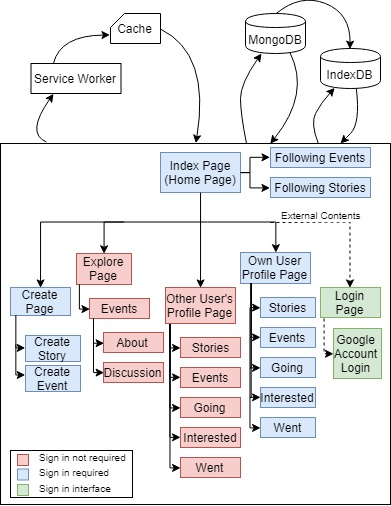
\includegraphics[width=8.5cm]{site_map.jpg}
    \caption{Demonstrates the flow of each web page in this PWA system along with the respective
    partial pages and external content pages.}
    \label{figure:site_map}
  \end{center}
\end{figure}
\begin{figure}[H]
  \begin{center}
    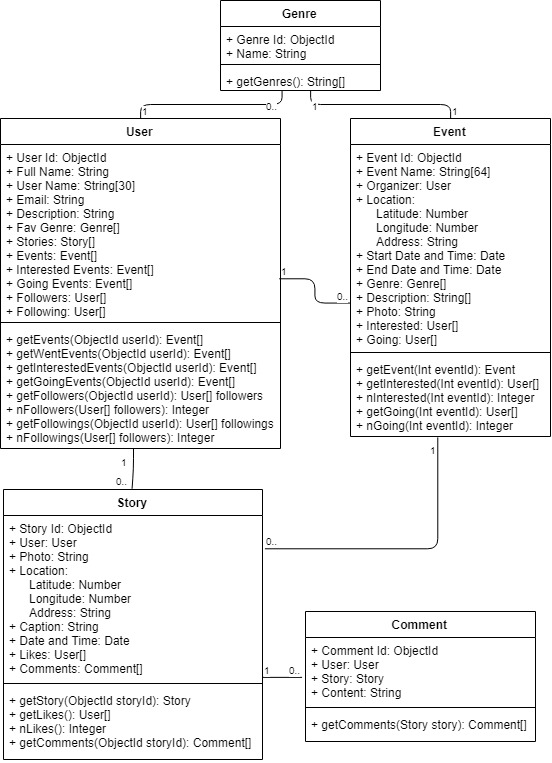
\includegraphics[width=15cm]{uml.jpg}
    \caption{Displays the structure of the database along with the types of content stored.}
    \label{figure:uml}
  \end{center}
\end{figure}


\end{document}
